\documentclass{article}                                                                           %basic LaTeX document type

\usepackage[margin=1.3in]{geometry}                                                     %set size of all margins
%\usepackage[left=1.3in, top=1in, right=1in, bottom=1in]{geometry}         %can set margin sizes which are not the same in this way

%\linespread{2}                                                                                         %option 1 for making text double-spaced
\usepackage{setspace}                                                                             %option 2 for making text double-spaced
\doublespacing                                                                                         %set double space

\usepackage{indentfirst}                                                                          %makes first paragraph of section indented (non-first are by default)
\setlength{\parindent}{25pt}                                                                     %set size of indentation (15pt is default)

\renewcommand\thesection{\Roman{section}}                                         %set capital Roman numeral section headings
\renewcommand\thesubsection{\thesection.\Alph{subsection}}                   %set capital Aramaic letters subsection headings
\renewcommand\thesubsubsection{\thesubsection.\arabic{subsubsection}} %set capital Arabic numbers subsubsection headings

\renewcommand*\thetable{\Roman{table}}                                              %set capital Roman numeral table numeration

\usepackage[explicit]{titlesec}                                                                  %package needed for next lines
\titleformat{\section}{\bfseries}{\thesection.}{1em}{\MakeUppercase{#1}}  %makes section headings bold and upper case characters
\titleformat{\subsection}{\bfseries}{\thesubsection.}{1em}{#1}                   %makes subsection headings bold
\titleformat{\subsubsection}{\itshape}{\thesubsubsection.}{1em}{#1}          %makes subsubsection headings in italics

\usepackage{lastpage}                                                                             %package which returns number of last page (same as number of pages)
\usepackage[figure,table]{totalcount}                                                        %package which counts the number of tables and/or figures

\usepackage{amsmath}                                                                            %enable `align' equation types

\renewcommand{\thefootnote}{\alph{footnote}}                                        %sets labeling of footnotes
\usepackage[]{footmisc}                                                                          %enables double spaced footnotes
  \renewcommand{\footnotelayout}{\doublespacing}                                  %double spacing of footnotes

%%% If you desire to place footnotes at the end of the document, uncomment these four lines and the two related near the end of this file
%\usepackage{endnotes}                                                                          %enables endnote page
%  \let\footnote=\endnote                                                                         %sets footnotes to endnotes
%  \renewcommand*{\theendnote}{\alph{endnote}}                                   %labels endnotes alphabetically
%  \renewcommand{\notesname}{Footnotes}                                            %renames endnotes title to footnotes

\usepackage{graphicx}                                                                             %enable figures
\usepackage{multirow}                                                                             %enable `multirow' capability in tables

\usepackage{caption}                                                                              %enables subfigures
\usepackage[labelformat=simple]{subcaption}                                           %enables subfigure captions
\captionsetup[table]{labelsep=newline,name=TABLE}                                 %sets table caption formatting options to meet NSE requirements
\captionsetup[figure]{name=Fig.,labelsep=period}                                     %sets figure caption options to meet NSE requirements
\renewcommand*\thesubfigure{(\alph{subfigure})}                                    %enables proper labeling of subfigures

\usepackage[colorlinks=true, allcolors=blue]{hyperref}                               %reference and citation hyperlinking linking

\usepackage{subfloat}
\usepackage{cite}
\usepackage{lineno, blindtext}

\DeclareMathOperator{\diff}{d}                                                                %can define operators to use in math mode, example in Eq. 2
\DeclareMathOperator{\erf}{erf}

\begin{document}

%Define fields for \maketitle

\title{Analysis of Using a Nuclear Fuel Cycle Simulator to Model a Nuclear Renewable Hybrid Energy System} %title of paper

\author{
\vspace{20mm}
\\Emma K. Redfoot,$^{\text{a},\ast}$ Dr. R.A. Borrelli \\[4pt] %list of authors, with corresponding author marked by asterisk
\textit{$^a$University of Idaho, Nuclear Engineering Department}\\[-10pt]       %affiliations of authors
\textit{995 University Blvd., Idaho Falls, ID 83401} \\[-5pt]
{$^\ast$Email: \href{mailto:redf3263@vandals.uidaho.edu}{redf3263@vandals.uidaho.edu}}}% email address for correspondence

\date{                               %instead of returning the date, this repurposes the \maketitle command to print the number of pages, tables, and figures
\vspace{40mm}
Number of pages: \pageref*{LastPage} \\
Number of tables: \totaltables \\
Number of figures: \totalfigures
}

\clearpage\maketitle
\thispagestyle{empty}


\pagebreak
%~\vfill
\begin{linenumbers}

\begin{abstract}
Growing concerns over the impact of fossil fuels on climate change have driven efforts to find low emissions sources of energy. In response, fluctuating renewable energy sources, such as solar and wind power, are growing to meet more of the electricity demand. However, maintaining reliable energy accessibility to the grid requires a stable, non-fluctuating source of power. Nuclear power plants provide nearly emissions-free, reliable energy to the grid \cite{IPCC}. To best reduce reliance on fossil fuels while ensuring reliable energy generation and profitability, nuclear renewable hybrid energy systems (NRHESs) focus on tightly coupling renewable generation with a nuclear power plant by co-locating the generation sources on an industrial park. The industrial park is comprised of at least the nuclear power plant, the renewable energy source, and some form of industrial process that consumes the energy not used by the grid. In this paper, we analyze the computational modeling approaches currently being pursued for NRHES. We further investigate similarities between Nuclear Fuel Cycle Simulators (NFCS) and NRHESs to determine how NRHES development can benefit from the development of NFCSs. This paper begins by reviewing past research on NRHES to determine the necessary functionality of modeling software. After determining the necessary software capabilities for an NRHES model, we discuss the characteristics of a NFCS. The characteristics found common to both systems include the desirability of a flexible modular design, open source, able to be coupled to external pieces of software, including economic modeling, optimization methods, and sensitivity analysis as well as results which are usable to technical and non-technical people alike.

%%%%%%%%%%%%%%%%%%%%%%%%%%%%%%%%%%%%%%%%%%%%%%%%%%%%%%%%%%%%%%%%%%%%%%%%%%%%%%%%
\end{abstract}

\vfill


\pagebreak
\section{Introduction}
Integrating non-emitting sources of power such as solar, wind, and nuclear provides a means of reducing greenhouse gas emissions. A Nuclear Renewable Hybrid Energy System (NRHES) is a power system which involves tightly coupling a nuclear power plant, a renewable, a battery, a natural gas plant, and an industrial process through co-locating the various facilities.  NRHESs are a proposed solution for allowing a nuclear power plant to fluctuate the electric output to the grid with a high penetration of variable energy sources. A NRHES seeks to minimize emissions such that they are significantly less than a renewable with load following by a natural gas plant \cite{Baker2016}.  Natural gas power plants, unlike nuclear and coal power plants, were built with flexibility in mind and are the typical means of load following \cite{MITEnergyInitiative2011}.  Understanding the impact of nuclear renewable hybrid energy systems in meeting future energy demand requires developing rigorous simulations to determine the system's economic prospects as well as its capacity to provide reliable, clean energy.

Renewable sources of energy and nuclear power both have the capacity to play an important role in mitigating climate change \cite {IPCC}. Due to the growth in variable energy generating sources, particularly wind and solar, grid flexibility has become a key driver in power system development \cite {Denholm2011}. Power system flexibility is defined by the Electric Power Research Institute (EPRI) as the "ability to adapt to dynamic and changing conditions, for example, balancing supply and demand by the hour or minute, or deploying new generation and transmission resources over a period of years \cite{EPRI2016}." Power system flexibility differs from load-following.  Load following is described as base-load power generator reductions \cite{Bragg-Sitton2014} or a power plant that adjusts its power output as demand for electricity fluctuates \cite{Masters2004}. Load following generally does not include following the predictable seasonal differences in electricity demand, but focuses more on the daily shifts. In the case of a NRHES, the nuclear power plant (NPP) will continue to run at full power output, allocating more or less electricity to the grid depending on demand.   Optimally, a NRHES will be able to respond to fluctuations in both seasonal and hourly demand. A NRHES combines power system flexibility with load following, adapting to dynamic conditions by changing the output of electricity to the grid.

First, we will provide a literature review covering both nuclear and non nuclear hybrid energy systems.  We will then discuss the ongoing research for modeling a NRHES to evaluate the important characteristics to include in a software model. Third, we will describe nuclear fuel cycle simulators (NFCS). Then we will analyze the similarities between the functionality needed to model a NRHES and a NFCS. While there are differences between the two systems, most obviously time scale and the need for a dynamic feedback response in a NRHES, the two physical systems share some common characteristics. NFCSs are at a more mature state of development, with some capacity to inform future development of NRHES software models.

\section{Background}
In order to ensure grid reliability (consistent electricity supplied to customers with a high penetration of fluctuating sources of power), traditional base load generating sources, such as nuclear power plants (NPPs), will need to increase their ability to fluctuate output to the electric grid \cite {Denholm2011}. For example, when wind decreases its electricity output, other sources of electricity need to respond quickly to make up for the loss. To supply electricity to a system including variable contributing sources, nuclear generation must be able to quickly increase and decrease its grid contribution. A NPP that is able to load follow would result in a reduction of unused energy while still ensuring grid reliability.

Reducing energy output below capacity for NPPs is sub-optimal due to the materials impacts of fluctuating the reactor and economically inefficient \cite{Nuclear2011}. NPPs are almost entirely comprised of fixed and sunk costs. The majority of the costs for nuclear are capital and operations (not including fuel), costs that do not depend on how much electricity is sold. As of 2010, nuclear fuel accounts for about 10\% of the levelized cost of electricity as compared to 70\%-80\% for natural gas \cite{IEA/NEA}. Due to the relatively small role the fuel plays in the overall costs of running an NPP operation, lowering the power output does not greatly reduce the generating costs. Fluctuating older nuclear power plants that were not designed for such maneuverability can accelerate the aging of the power plant, causing physical and economic damage \cite{Nuclear2011}. Assuming economic conditions in the energy sector remain constant, NPPs must run at near full capacity to compete economically and avoid materials degradation.

\subsection{Hybrid Energy Systems}
A Hybrid Energy System (HES) is a coupled means of energy generation generally including at least one renewable and one conventional energy source \cite {Ibrahim2011}. These systems provide electricity through multiple generation sources working together, unlike co-generation which is simultaneously produces heat and power \cite{Rosen2005}." Traditional HES generate only a single product, electricity, from multiple sources. Co-generation systems create multiple outputs, such as electricity and heat, from a single energy generation source. HES have been implemented all over the world in stand-alone and grid connected systems to balance the variability of solar and wind \cite {Garcia2015, Qi2014, Shin2015, Nixon2012, Adaramola2014, Goodbody2013, BorgesNeto2010, McGowan1996}. In standalone systems, the renewable generating source is generally combined with a diesel generator, a battery, or both. The operational goal of all HES is to pair fluctuating energy generation sources with consistent energy producers and/or storage mechanisms in order to have a reliable electrical generating system.

Traditional HES generate energy in the location where it is used \cite {Shin2015, Nixon2012, Adaramola2014, Goodbody2013, McGowan1996}. For example, Shin et al. (2015) optimized meeting the energy needs of the Deokjeok Islands, part of South Korea, which are disconnected from the grid, using renewable power sources and diesel generators. Different approaches for HES as a means of electricity access for people in rural regions or developing nations have been discussed in Borges et. al. (2010) where biogas and photovoltaics (PVs) provide energy to the surrounding region \cite{BorgesNeto2010}. Nixon et. al. (2012) evaluated multiple solar-biomass systems for decentralised power production \cite{Nixon2012}. Adaramola et. al. (2014) used the Hybrid Optimization Model for Electric Renewable (HOMER) computational tool to model a wind and solar HES system in southern Ghana \cite{Adaramola2014}. Rehman et. al. (2010) studied PV-diesel-battery HES for a rural region of Saudi Arabia \cite{Rehman2010}. Mahmoud et. al. (2004) discussed the economic benefits of a PV-diesel generator system hooked up to the electric grid \cite {Mahmoud2004}. The above research describes multiple inputs single output (MISO) systems\cite{Garcia2013}.A significant body of research literature describes off-grid situated hybrid energy systems, demonstrating that HES can provide reliable energy.


In contrast to multiple means of energy generation producing one product, multiple input multiple output systems (MIMO) use any excess energy not used by the grid at a given moment to generate other products to increase profitability \cite {Garcia2013}. Figure 1 has been constructed to demonstrate the differences between a system where electricity generation is the sole purpose (MISO) versus a system that produces electricity and another good, such as desalinated water or hydrogen. The sources of energy are gray while the energy sinks are white. Both diagrams differ from co-generation because they illustrate more than one source of energy contributing to the system. The primary benefit of a MIMO system is a diversified income source, thus the system is better economically shielded from fluctuations in electricity prices. Both types of systems attempt to provide reliable energy to the grid while incorporating a fluctuating source of energy.

 While the current microgrid hybrid energy system tools, such as HOMER, should be evaluated when determining the characteristics for a NRHES model, there are major differences between small, home-owner projects, and large industrial scale projects. The large industrial scale projects require more thorough physics models, especially when they are including an industrial process. There has been significant research done on small scale MISO HES.  There has been less work done on a large HES which has a major goal of functioning as a backup source to a fluctuating renewable. The focus of this paper is exclusively on the large HES.

 \begin{subfigures}
\begin{figure*}[h!]
\centering
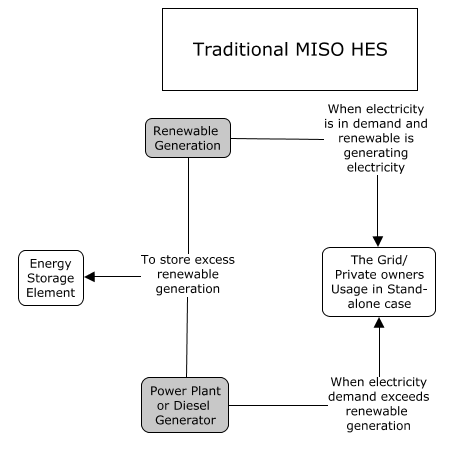
\includegraphics[width=.75\textwidth]{TraditionalHES.PNG}
\caption{\small \sl Traditional HES are smaller systems meant to provide power at the location where the electricity is made.  They have traditionally balanced fluctuating sources of power with reliable sources of electricity.}
\end{figure*}

\begin{figure*}[h!]
\centering
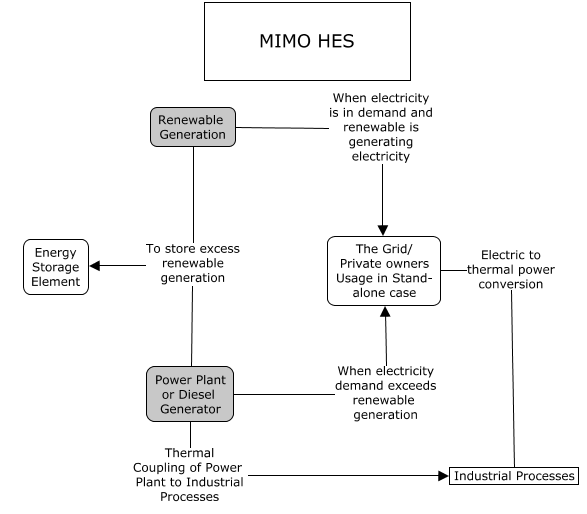
\includegraphics[width=.75\textwidth]{MIMO_HES.PNG}
\caption{\small \sl Figures 1a and 1b compare the MISO and MIMO configurations demonstrating the differences between traditional hybrid energy systems that are focused on generating reliable electricity and non-traditional hybrid energy systems which have the added objective of generating an additional product.  While many of the elements are the same, the MIMO system includes an industrial process which is either thermally or electrically coupled.}
\end{figure*}
\end{subfigures}

\subsection{Nuclear Renewable Hybrid Energy Systems}

A Nuclear Renewable Hybrid Energy System (NRHES), as defined by Bragg-Sitton et al. (2014) is the "tighter coupling of nuclear and renewable energy sources in a manner that better optimizes energy use for the combined electricity, industrial manufacturing, and transportation sectors capable of apportioning thermal electrical energy to first meet the grid demand (with appropriate power conversion systems), then utilizing excess thermal and, in some cases, electrical energy to drive a process that results in an additional product \cite {Bragg-Sitton2014}".  One potential benefit of co-locating the various facilities in the NRHES is optimizing the system to minimize cost to the NRHES as a whole while increasing economic resilience by diversifying both the means of generating energy as well as the products produced. For example, if natural gas prices increase, there could be less reliance on the natural gas plant and more focus on storage.  On a more short term perspective, if electricity prices are negative, the energy produced by the NRHES can be diverted to the industrial process. Other benefits include decarbonizing both the electric grid as well as industrial processes through the coupling with the nuclear power plant. Furthermore a NRHES is both a flexible and reliable system increasing the overall flexibility and reliability of the grid as a whole.

While there are definite benefits of a NRHES, there are clear challenges to implementation. The main drawback of co-locating the various generation sources and the industrial processes is the increased complexity of the system.  While there are cases of thermal coupling of nuclear power plants internationally; in Norway, Switzerland, Germany, and Canada \cite{Verfondern};  there have never been any nuclear thermal couplings thus far in the United States.  The low level state of development as well as the lack of experimental data in the United States suggest a demand for rigorous technical work.  There are concerns surrounding the regulatory oversight with a thermally coupled NRHES and whether it falls under the Nuclear Regulatory Commission's umbrella. There are multiple economic concerns. A NRHES would need contracts that ensure all of the participants in the NRHES are profitable if the system as a whole is profitable. Further policy and economics investigations need to analyze when running the NRHES in an economically optimal way is considered market manipulation. So, while there are motivations to analyze the benefits of a NRHES, those benefits always need to be analyzed with the context of the major economic, technical, and excess overhead costs also associated with a complex interconnected system.

The additional products include, but are not limited to: synthetic fuel, desalinated water, hydrogen production, metals production, and heat pumps \cite{Bienvenue2015}. The nuclear power plant diverts the energy it generates between the grid and the industrial process to maximize profit or minimize costs. The system can allocate energy based on the market value of each of the multiple outputs produced. In the case of a nuclear power plant coupled with a desalination plant, for example, if the price of electricity is low, more thermal and/or electric energy can be diverted to generate more clean water at a higher profit \cite {Chen2016}. The costs of running a dynamic system, such as the case with a NRHES, include additional wear and tear, decreased thermal efficiency, and increased complexity of operations \cite{Garcia2013}. While there is ongoing economic research into NRHES, the total costs of any particular system have yet to be determined \cite{Rabiti2015}.

There have been no physical demonstrations to date of NRHES. Therefore, research has largely focused on computational modeling to determine the feasibility and optimization of coupling elements \cite{Boardman2013, Shropshire2012}. Creating a model for a NRHES is important for determining technical as well as economic optimization of the elements that could comprise such systems. Models are used as a means for forecasting limitations and functionality in specific conditions in order to ensure safety and reliable electricity production. Computational models can provide feedback regarding which NRHES models are worth pursuing given the expected profitability. A NRHES simulator could help inform policy and technology decisions.

Our literature review revealed that a lot of work on NRHES is in the design and analysis stage \cite{Boardman2013, Shropshire2012}. Research is focused on developing a model that can dynamically simulate the contributions of variable energy sources, the constraints of fluctuating electricity demand, and thermal/electrical power demands for various industrial processes. The models focus on answering questions regarding minimizing costs for each of the components comprising the NRHES. In order to move forward with development of any NRHES,  such systems must demonstrate that they can be profitable and can reliably respond to fluctuating electricity production and demand \cite{Rabiti2015}.

An ongoing effort at Idaho National Laboratory (INL), Argonne National Laboratory (ANL), and Oak Ridge National Laboratory (ORNL) focuses on modeling a generic NRHES.As part of this study, we have gained from some input from INL researchers in the hybrid energy system division who are leading experts in the field. The generic model will test the economic viability of a NRHES to determine how future development should be pursued. The industrial plant combines a nuclear power plant, a wind farm, a natural gas power plant, a battery, and a high temperature steam electrolysis hydrogen production facility. More component models will be developed in the future that can allow for the comparison of various industrial customers\cite{Harrison2016}. The chosen renewable source, a wind farm, models a highly stochastic system due to the unpredictable nature of wind generation \cite{Chen2016_wind}. The model optimizes the sizes of the nuclear power plant, the natural gas plant, and the battery. The objective is to choose the NRHES configuration that minimizes costs while meeting set emissions and grid reliability expectations.

NRHES sit in an interesting location in computational modeling. Many tools have been developed to model nuclear reactors and the nuclear fuel cycle as demonstrated in the nuclear fuel cycle simulators shown in Figure 2. Many tools have also been created to model and optimize non-nuclear hybrid energy systems (HOMER, Hybrid2, SOLSIM, SOMES, ARES, RAPSIM, HOGA)\cite {Bernal-Agustin2009}. Modelica and Excel, while neither are specifically HES or NRHES tools, have been used to model both nuclear and non-nuclear hybrid energy systems \cite{Shropshire2012, Chen2016, Binder2014, Garcia2015, Epiney2016}. HES tools are typically bought for microgrid standalone systems. The main challenges to applying HES software to a NRHES are the scale of the system being modeled and including the grid demand. Small microgrid systems do not include large industrial processes which require thorough physics models.

\section{State of the Art}
There are criteria that make a tool better for modeling a NRHES. In order to select a tool to model a NRHES, it is necessary to understand what characteristics a model must possess in order to provide accurate information. For example, as discussed below, it is important for a NRHES model to incorporate the dynamic nature of the system. Understanding the differences among the underlying mathematical models as well as the software functionality is essential in determining whether and how a nuclear fuel cycle simulator (NFCS) will be useful to NRHES modeling.
As mentioned above, the model currently under development by the Oak Ridge National Laboratory, the Argonne National Laboratory, and the Idaho National Laboratory has reviewed the essential characteristics for a computational model of a NRHES. Rabiti et al. (2015) discusses the important elements of a NRHES computational model in detail, describing the basic requirements of the software as a "computational representation of the thermal, mechanical, chemical, and electrical processes in the systems as process units, reactors, manufacturing plants, and energy delivery (to the appropriate point of interface with the market transaction, such as an electricity bus, or a product depot or distribution terminal where a commodity price is established)"\cite{Rabiti2015}. The model in development by the national laboratories combines RAVEN (Reactor Analysis and Virtual Control Environment) for the stochastic aspects of the system and Modelica for modeling the various components in the NRHES.

\subsection{Modelica}
Modelica is a widely used open source language for modeling large and complex systems composed of smaller component models. It is particularly optimized for modeling dynamic systems. Modelica has powerful libraries, such as Thermopower, that include the thermohydraulic modeling tools required for modeling mass flows in energy systems \cite{Binder2014}. The language is well-maintained, giving it the added benefits of having up-to-date documentation and a community that can provide support. Typically Modelica is run on the Dymola developer environment, a private tool developed by the creator of Modelica, Dr. Hilding Elmquist. Another option for running the Modelica language is the open source OpenModelica environment.

A Modelica HES model developed in Binder et. al. (2014) includes a nuclear reactor, two steam cycles, a chemical plant, and an electrical component \cite{Binder2014}. The products of this Modelica NRHES model are synthetic fuel and electricity. The model includes the ramp up stage when the reactor initially starts or is increasing from a lower load. The steam generator connected to the NPP determines which of its turbines to use depending on electricity demand, the 60\% turbine, the 30\% turbine, or the 15\% turbine, which can be used in unison. A pressure relief valve releases excess energy unused by the turbines. The wind generation is modeled using the Western Wind dataset from the National Renewable Energy Laboratory (NREL) for an unspecified region in Idaho. Each component in the model was tested individually before being combined. Using the individual component models, verifications were made for the system as a whole. The startup transient state of the model took much greater computation time due to the complex interrelations of the components. Generally, running a model of a NRHES in Modelica requires a control algorithm, a differential equation that controls how the dynamic system allocates heat. The profitability control algorithm can be adjusted to incorporate varying parameters such as the price of electricity or the cost of natural gas. The study concluded that Modelica, due to its ability to evaluate control algorithms, is an effective tool for dynamically modeling a HES. As a tool that is optimized for large dynamic systems, Modelica has been used more than any other tool to model NRHES at this point.

\subsubsection{RAVEN}
The RAVEN tool was initially built for probabilistic risk assessment. RAVEN, as a probabilistic tool, can do parametric and stochastic analyses of systems\cite{RabitiRAVEN}. For the NRHES, RAVEN is used to run different wind energy generation paths in order to generate a statistically fair representation of how renewables, in this case wind power, would likely function over any given hour. RAVEN can be used to generate the most generic seasonal wind generation over a week. A typical week can be extrapolated to represent a given season. The process can be repeated over the different seasons, which can be extrapolated to represent a year. Using synthetic generated data instead of historic data avoids the critique that the model only represents past behavior and is thus inapplicable to future trends \cite{redfoot_epiney_2016}. RAVEN can also be used to determine high-risk time series samples to ensure that high risk scenarios are accounted for in the study. RAVEN can also do probabilistic assessments such as loss of load probability and sensitivity to uncertainty analysis.

From our literature review, we conclude that any future modeling efforts for a NRHES would benefit from complimenting the ongoing modeling effort. Currently, all of the physics models for the NRHES are built in Modelica. To benefit from the work already done, any additional software would need to be able to easily communicate with the Modelica modeling language.  The model would benefit from a tool that would communicate with other chemical and utility standard physics modeling tools. Future work would benefit from coupling with other physics modeling tools, allowing groups to take advantage of the existing infrastructure while using their physics model of choice.

\subsection{Distinct Capabilities}
There are certain characteristics of a physical NRHES which a computational model would need to have to be a reasonable assessment of the system as a whole. Table I below demonstrates the functions which are most commonly incorporated in a model. We discuss dynamic modeling explicitly as it is the capability highly valued in a NRHES that is not nearly as important in a NFCS. The below discussion details the extensive work that has been done determining why a dynamic system is important to a NRHES.

In Garcia et. al. (2013) and Du et. al. (2014), a dynamic approach to modeling hybrid energy systems (HES) is applied in order to appropriately address the impacts of flexible operation of the system due to variable renewable generation \cite{Garcia2013, Du2014}. In Du et. al. (2014), two optimization problems are addressed: the first minimizes variability in the HES through optimizing components of the HES system, and the second imposes operating and capital costs on the design variables. Garcia et. al. (2013) has a two-part series. The first applies and analyzes performance of a dynamic approach to modeling some of the physical components of a traditional and an advanced (produces goods besides electricity) HES. The second paper focuses on economic effects using a dynamic approach, as opposed to time series or statistical analysis. Overall, both parts of the series focus on how a dynamic approach better models the high level of variability of a HES for output generation and profitability maximization \cite{Garcia2013}. The costs of operating in a flexible manner, dynamically allocating resources between multiple coupled systems, are substantial enough to require a simulation that precisely models the variability of the system \cite{Garcia2013, Shropshire2011, Locatelli2015}. The dynamic modeling at this point focuses on the dynamic transfer of energy to different sources, and how this impacts the economics and grid reliability. The physical impacts of the grid system have not yet been included in the model \cite{Harrison2016}.  The dynamic allocation of the heat and electricity depending on the renewable generation and the grid demand is an essential characteristic of a NRHES.  Including factors such as how quickly the NRHES will be able to switch between providing energy to the industrial facility and the grid will impact determining the economic and physical values of the model.

Table I displays the characteristics routinely included in modeling a NRHES along with their citations.

\begin{table}[h!]
\centering
\caption{References for Each NRHES Model Function}
\begin{tabular}{ ||c | c|| }
 \hline
 NHRES Model Function & Paper \\ [0.5ex]
 \hline \hline
 Dynamic & \cite{Garcia2013, Du2014, Kazimi, Garcia2016}\\
 \hline
 Sensitivity Analysis & \cite{Shropshire2011, Rehman2010, Adaramola2014, Chen2016}\\
 \hline
 Optimization of components & \cite{Chen2016,Ozcan2016, Forsberg2009,Garcia2015,Aumeier2011}\\
 \hline
 Stochastic Model of Renewables & \cite{Rabiti2015, Garcia2016,Locatelli2015}\\
 \hline
 Grid Demand model & \cite{Forsberg2013, Garcia2016,Garcia2013,Ruth2014,Chen2016}\\
 \hline
  Economic FOMs & \cite{Garcia2016,Chen2016,Rabiti2015,Epiney2016,Bragg-Sitton2014}\\
 \hline
\end{tabular}
\label{table:1}
\end{table}

The table displays the characteristics found most commonly in the NRHES literature review.  The six characteristics are beneficial to modeling the important physical characteristics as well as indicators of successful implementation of a NRHES.  Each of these characteristics have been included in previous studies, and thus have some already proposed approaches.  The characteristics can be studied in greater detail in order to determine if they satisfactorily model the system.

\section{Nuclear Fuel Cycle Simulators}

This section identifies basic properties of nuclear fuel cycle simulators and assesses their distinct capabilities. Figures 2a and 2b display many of the currently used NFCSs. The fuel cycle simulators are the central nodes in these figures, with the tools for computing some of the basic descriptive qualities of a fuel cycle branching off. The computational attributes that are often included in a NFCS include: mass flows, reactor physics, thermal hydraulics, reprocessing, waste management, risk management, and economics. While different NFCSs were initially optimized for a variety of applications, there is a lot of overlap in their functionality \cite {Guerin2009}. Because NFCSs are attempting to model the same thing, the nuclear fuel cycle, the models include some means of tracking the fuel composition as they move through the fuel cycle. The different fuel cycle simulators generally have the ability to simulate fleets of nuclear reactors with the associated fuel cycle. As can be seen in figues 2a and 2b, there are a good number of NFCSs which all have different functionality and dependencies.

\begin{subfigures}
\begin{figure*}
\includegraphics[width=\textwidth]{NFCS_US.PNG}
\caption{\small \sl This figure displays the nuclear fuel cycle simulators developed in the United States, though they are not necessarily specifically built to demonstrate the development of a US fuel cycle. This figure does not include all nuclear fuel cycle simulators or their dependencies.  The figure demonstrates some of the complexity of the current Nuclear Fuel Cycle Simulator options. The figure demonstrates the types of tools NFCSs depend on, thereby suggesting some of their functionality.}
\end{figure*}

\begin{figure*}
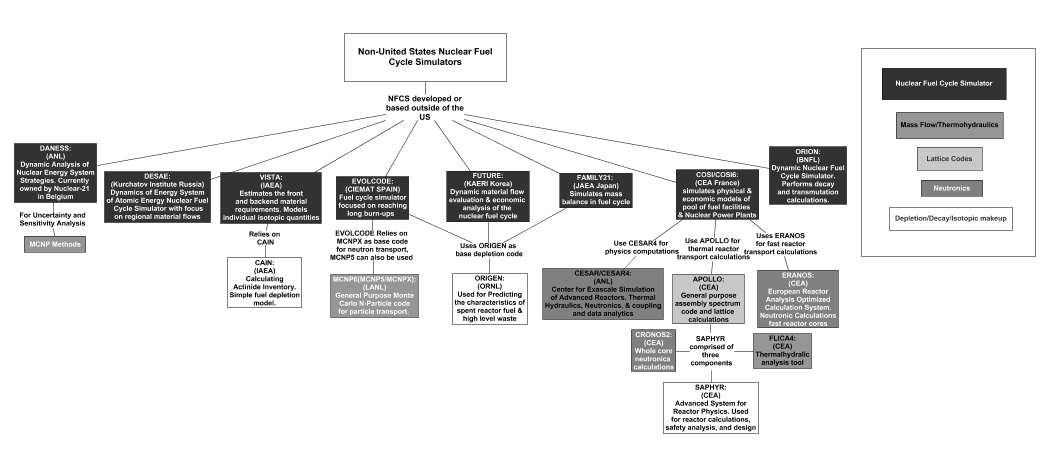
\includegraphics[width=\textwidth]{NFCS_non_us.PNG}
\caption{\small \sl This figure displays the nuclear fuel cycle simulators developed outside of the United States.The full relationship between the various computational tools may not be covered.  The literature is lacking in descriptions of the evolution and dependencies of the computational tools.}
\end{figure*}
\end{subfigures}

The major difference between many of these nuclear fuel cycle simulators is the ability to model discrete facilities and fuel batches versus modeling continuous mass flows throughout the fleet of facilities operating in an identical fashion. In the case of the fleet modeling, the average value for each of the facilities is assumed. The discrete model requires more information while providing a more detailed analysis. The discrete model is, however, more computationally complex and expensive.

In "Modeling the Nuclear Fuel Cycle," Juchau et al. (2010) describe four functions as necessary for a NFCS to meet the desired qualities of an organization proposed at the time called the Simulation Institute for Nuclear Enterprise Modeling and Analysis \cite{Juchau2010}. The four functions, which are reiterated in other synopsis of Nuclear Fuel Cycle Simulators \cite{Wilson2012, NEA2012} include: discrete facilities and material tracking, uncertainty analyses, ability to optimize, and open and accessible with high quality documentation to ensure collaboration. Juchau et al. (2010) reviews the nuclear fuel cycle simulator tools CAFCA, COSI, CEPMNFC, DANESS, NFCSim, VEGAS, VISION, NFCSS, and GENIUS 1. His conclusion is that many of these tools have overlapping functionalities, partially due to the proprietary nature of at least parts of each.

One of the reasons why there are so many nuclear fuel cycle simulators is that many of the countries that currently have NPPs have designed their own simulators. While some NFCSs, such as DANESS, are used in multiple countries, many countries have developed their own NFCSs.  DANESS can be seen in figures 2a and 2b as it has been developed and used both in and out of the US. Figure 2b depicts the non-US NFCSs along with some of their software dependencies. Most of the fuel cycle simulators are not open source or available for download; thus, each nation tends to have proprietary software. As discussed with University of Illinois Professor and developer of the Cyclus nuclear fuel cycle simulator, Dr. Kathryn D. Huff, it is also often more efficient, both in terms of time spent as well as better integration, if the different functions are designed by the same team (\cite{redfoot_huff_2016}). Integrating components from one system into a new system can often be more challenging than building the function from scratch. While sharing code can be challenging amongst various program, some calculations or libraries are commonly used by NFCSs. For example, Figure 3 depicts EVOLCODE, FUTURE, and FAMILY21 as all relying on Origen.

The 2016 Electric Power Research Institute report "Program on Technology Innovation: Assessment of Nuclear Fuel Cycle Simulation Tools" takes a commercial software architecture approach to analyze sixteen NFCSs.  The NFCSs are evaluated based on functionality, usability, reliability, performance, and supportability. Of the sixteen NFCSs included, only six NFCSs garnered responses: CAFCA, COSI6, CYCLUS, DANESS, ORION, and VISION. As is true with other NFCS Benchmarking papers, the EPRI report used feedback from users of the NFCS \cite{EPRI2016}.  The data in the report is anonymous, making it difficult to distinguish which of the NFCSs particularly stood out for each of the categories. The overall approach of analyzing the software based on commercial software architecture criteria, with many subcriteria, is an important assessment for the adoption of the tool by end users. Some of the criteria the end users involved in the survey viewed as being helpful included: parallel processing, open-source, the flexibility to model complex scenarios, uncertainty/sensitivity analysis, economic capabilities, visual tools, and ability to track many nuclides.

The Nuclear Energy Agency's 2012 report "Benchmark Study on Nuclear Fuel Cycle Transition Scenarios Analysis Codes" compares nuclear fuel cycle simulators in three scenarios: light water reactors with direct spent fuel disposal, reprocessing light water reactor fuel, and the transition between light water reactors and fast reactors \cite{NEA2012}. The NFCs included in the study include COSI6, DESAE2.2, EVOLCODE2.0, FAMILY21, and Vision2.2. The benchmark focused on the common characteristics of each of the codes to determine the similarity of the outcomes when modeling the same scenarios. Depletion values of heavy element material flows are directly compared between the simulators, with numerical data included in the report. The Benchmark study concludes that some of the key differences between the various NFCSs include the ability to model discrete batches of fuel as opposed to annually averaged batches, with increased complexity the outcomes between the various NFCSs diverge more, and the different simulators use different physics models for decay and depletion calculations. This report focuses on determining the differences in the outcomes when modeling the same system, so it really evaluates the fuel characterization and depletion abilities of the NFCSs. This benchmark does not focus on the differences in capabilities between the NFCSs, such as economic modeling capabilities or a visual tool.


From the literature reviewed and figures 2a and 2b, nuclear fuel cycle simulators have certain common characteristics. Generally, there is a means of tracking the nuclear fuel materials and the composition of those materials using an associated decay software. NFCSs should generally be flexible and able to include new components, able to incorporate other pieces of software, able to do an uncertainty analysis, and accessible to technical and non technical audiences alike. Some of the characteristics discussed as applying to a NFCS also apply to a NRHES as will be discussed in the following section.

\section{Analysis}
The underlying structure of passing materials between various facilities is similar enough between nuclear materials in a fuel cycle and heat or electricity flow in a NRHES that a NFCS could model a nuclear renewable hybrid energy system. In the case of a NRHES model, the facilities are the NPP, the renewable, and the industrial process at least.  In the case of the nuclear fuel cycle, the facilities are the steps in the given fuel cycle. Noting the capabilities found desirable by end users in the EPRI 2016 report, all of the criteria besides from the ability to track many nuclides could also be applied to a NRHES. Both systems are time dependent and include uncertainty measures. Many of the uncertainty measures found in NFCSs are the same for a NRHES including O\&M costs, water costs, and challenges in siting a nuclear power plant. Optimally, both systems would be:
\begin{itemize}

\item flexible so that new component models and specific regional characteristics could easily be added
\item well documented and accessible
\item include uncertainty/sensitivity analysis capabilities
\item usable by technical and non technical people alike to address policy decisions.

\end{itemize}

If a NFCS were to model a NRHES, it would need to be able to function in a dynamic or quasi dynamic state to capture the dynamic nature of the NRHES.  The nuclear fuel cycle does not require materials to be exchanged nearly as regularly as a nuclear hybrid energy system and with as inconsistent of quantities. The dynamic impacts on the physical system would need to be included in order to generate a meaningful model of a NRHES. The stochastic aspect of the renewables components of a NRHES would also require either external coupling with a tool able to model randomness such as RAVEN or the use of real time data from a specific region. The dynamic and stochastic components of modeling a nuclear hybrid energy system would take some work to incorporate.

Many of the features commonly found in a NFCS would not be needed in a NRHES model.  There would be no need to model a fleet of NRHESs at this point in development, so a system would have to be able to model discrete facilities.  The reactor calculations, such as burnup, would not be needed for a NRHES.  The back end of the fuel cycle, such as models for reprocessing and long term waste storage would also not be applicable at this point to a NRHES model.  The primary qualities that would be used are optimization methods, economic evaluation, and means of exchanging materials in a system. The optimization methods and economic evaluation can be applied externally from the primary modeling tool.  Therefore, this preliminary analysis does not find a major reason to pursue modeling a NRHES with a NFCS.

\section{Summary Remarks}
While nuclear fuel cycle simulators share some similar underlying characteristics with a nuclear renewable hybrid energy system, there is significant enough differences for software to likely be incongruent.  NFCSs are not continuous mass flow systems, they have much larger time scales than NRHES, and they are not run in a dynamic fashion. The major challenge in modeling a NRHES with a NFCS is including the dynamic aspects of the system and how that will affect the overall costs of the system. So to conclude, NRHES modeling as it progresses can benefit from NFCS development by incorporating desirable software characteristics such as being open source, easy to incorporate new components, flexible, including economic tools and sensitivity/uncertainty tools. Future work on the current NRHES models could benefit from the ability to be coupled with external tools for the physics modeling for the various industrial components. The current model under development at the national laboratories already has sensitivity and uncertainty analyses due to the coupling of the system with RAVEN as well as economic analysis. Future work on NRHES modeling could include developing a visual tool, making the model more flexible for including other sources of software, and progressing the planned release of the model as an open source tool.


\end{linenumbers}

%%%%%%%%%%%%%%%%%%%%%%%%%%%%%%%%%%%%%%%%%%%%%%%%%%%%%%%%%%%%%%%%%%%%%%%%%%%%%%%%

\pagebreak
\section*{Acknowledgments}

Thank you to Dr. Shannon Bragg-Sitton, Dr. Cristian Rabiti, Dr. Aaron Epiney, Dr. Jong Suk Kim, and Dr. Kathryn Huff for their time and insight.

\pagebreak
\bibliographystyle{ans_js}                                                                           %custom ANS journal submission template bibliography style
\bibliography{bibliography}

%%% If you desire to place footnotes at the end of the document, uncomment these two lines and the four related near the beginning of this file
%\pagebreak
%\theendnotes

\end{document}
